\documentclass[twoside, 11pt]{exam}

\usepackage[T1]{fontenc}
\usepackage[utf8]{inputenc}
\usepackage[dutch]{babel}

\usepackage[font={small,sf},labelfont={bf},labelsep=endash]{caption}
\usepackage{fouriernc}
\usepackage[detect-all, binary-units, separate-uncertainty=true,
            per-mode=symbol, retain-explicit-plus, range-phrase={ tot },
            list-final-separator={ en }, output-decimal-marker={,}]
            {siunitx}

\usepackage{setspace}
\setstretch{1.2}

\setlength{\parskip}{\smallskipamount}
\setlength{\parindent}{0pt}

\usepackage{geometry}
\geometry{a4paper, vmargin=3cm, inner=3cm, outer=2cm, head=14pt}

\usepackage{float}

\usepackage[fleqn]{amsmath}
\numberwithin{equation}{section}
\numberwithin{figure}{section}

\usepackage{graphicx}
\graphicspath{{Figures/}}
\usepackage{subfig}

\usepackage[svgnames]{xcolor}
\usepackage{tikz}
\usepackage{tikz-3dplot}
\usepackage{pgfplots}
\usetikzlibrary{plotmarks,circuits.ee.IEC,pgfplots.groupplots,external,calc}
\pgfplotsset{compat=1.3}

\usepackage{minted}
\usepackage{amsthm}
\usepackage{relsize}
\usepackage{xspace}
\usepackage{url}
\usepackage{sansmath}
\usepackage{titling}


\theoremstyle{plain}
\newtheorem*{note}{Note}


\newcommand{\figref}[1]{Figuur~\ref{#1}}

\newcommand{\hisparc}{\textsmaller{HiSPARC}\xspace}
\newcommand{\kascade}{\textsmaller{KASCADE}\xspace}
\newcommand{\sapphire}{\textsmaller{SAPPHiRE}\xspace}
\newcommand{\jsparc}{\textsmaller{jSparc}\xspace}
\newcommand{\hdf}{\textsmaller{HDF5}\xspace}
\newcommand{\aires}{\textsmaller{AIRES}\xspace}
\newcommand{\csv}{\textsmaller{CSV}\xspace}
\newcommand{\python}{\textsmaller{PYTHON}\xspace}
\newcommand{\corsika}{\textsmaller{CORSIKA}\xspace}
\newcommand{\labview}{\textsmaller{LabVIEW}\xspace}
\newcommand{\dspmon}{\textsmaller{DSPMon}\xspace}
\newcommand{\daq}{\textsmaller{DAQ}\xspace}
\newcommand{\adc}{\textsmaller{ADC}\xspace}
\newcommand{\adcs}{\textsmaller{ADC}s\xspace}
\newcommand{\Adcs}{A\textsmaller{DC}s\xspace}
\newcommand{\hi}{\textsc{h i}\xspace}
\newcommand{\hii}{\textsc{h ii}\xspace}
\newcommand{\mip}{\textsmaller{MIP}\xspace}
\newcommand{\hisparcii}{\textsmaller{HiSPARC II}\xspace}
\newcommand{\hisparciii}{\textsmaller{HiSPARC III}\xspace}
\newcommand{\pmt}{\textsmaller{PMT}\xspace}
\newcommand{\pmts}{\textsmaller{PMT}s\xspace}
\newcommand{\gps}{\textsmaller{GPS}\xspace}

\DeclareSIUnit{\electronvolt}{\ensuremath{\mathrm{e\!\!\:V}}}

\DeclareSIUnit{\unitsigma}{\ensuremath{\sigma}}
\DeclareSIUnit{\mip}{\textsmaller{MIP}}
\DeclareSIUnit{\adc}{\textsmaller{ADC}}

\DeclareSIUnit{\gauss}{G}
\DeclareSIUnit{\parsec}{pc}
\DeclareSIUnit{\year}{yr}


%% Document style definitions

% macros and commands
\newcommand{\shorttitle}[1]{\def\theshorttitle{#1}}
\newcommand{\docindex}[1]{\def\thedocindex{#1}}
\newcommand{\version}[1]{\def\theversion{#1}}
\newcommand{\setsectionstyle}[2]{
  \colorlet{seccolor}{#1}
  \def\thesectiontitle{#2}
}

\newcommand{\setdocumentstyle}[4]{
  \setsectionstyle{#1}{#2}
  \docindex{#3}
  \shorttitle{#4}
}

% document types
\newcommand{\docalgemeen}[2]{\setdocumentstyle{red}{Algemeen}{#1}{#2}}
\newcommand{\docinstallatie}[2]{\setdocumentstyle{Gold}{Detector installatie}{#1}{#2}}
\newcommand{\docdetector}[2]{\setdocumentstyle{blue}{Detector}{#1}{#2}}
\newcommand{\docweerstation}[2]{\setdocumentstyle{LightSlateGray}{Weerstation}{#1}{#2}}
\newcommand{\docbliksem}[2]{\setdocumentstyle{orange}{Bliksem}{#1}{#2}}
\newcommand{\docanalyse}[2]{\setdocumentstyle{DarkViolet}{Data analyse}{#1}{#2}}
\newcommand{\docwerkblad}[2]{\setdocumentstyle{ForestGreen}{Werkbladen}{#1}{#2}}
\newcommand{\docdocent}[2]{\setdocumentstyle{DarkKhaki}{Uitwerkingen}{#1}{#2}}
\newcommand{\docopdrachten}[2]{\setdocumentstyle{Silver}{Opdrachten}{#1}{#2}}
\newcommand{\docrecept}[2]{\setdocumentstyle{Navy}{Recept}{#1}{#2}}

\pgfmathsetlengthmacro\stylemarginsep{+1cm}
\pgfmathsetlengthmacro\stylethumbsep{+.75cm}

\newcommand{\rightthumb}{
\begin{tikzpicture}[remember picture, overlay]
  % vertical line
  \draw[seccolor]
    ($(current page.north east) + (-\stylemarginsep, -.5cm)$) --
    ($(current page.south east) + (-\stylemarginsep, .5cm)$);

  % thumb
  \fill[seccolor]
    ($(current page.north east) +
      (-\stylemarginsep, -2cm -\thedocindex * \stylethumbsep)$)
      rectangle +(.5cm, -.5cm);
\end{tikzpicture}
}

\newcommand{\leftthumb}{
\begin{tikzpicture}[remember picture, overlay]
  % vertical line
  \draw[seccolor]
    ($(current page.north west) + (\stylemarginsep, -.5cm)$) --
    ($(current page.south west) + (\stylemarginsep, .5cm)$);

  % thumb
  \fill[seccolor]
    ($(current page.north west) +
      (\stylemarginsep, -2cm -\thedocindex * \stylethumbsep)$)
      rectangle +(-.5cm, -.5cm);
\end{tikzpicture}
}

\renewcommand{\maketitle}{
  \suppressfloats

  \begin{titlepage}
  \thispagestyle{\defaultstyle}
  \let\endtitlepage\relax
  \begin{tikzpicture}[remember picture, overlay,
    titlebox/.append style={seccolor, fill, text=white, minimum height=1cm,
      font=\sffamily\huge, draw=none},
    authorbox/.append style={minimum height=.5cm, font=\sffamily}]

    \node[titlebox, anchor=north west, shift={(3cm, -1cm)}] at
      (current page.north west) {\thesectiontitle};

    \node[anchor=north west, shift={(2.83cm, -2cm)}] at
      (current page.north west) {
\includegraphics[scale=.8]{../HiSPARC_header}};

    \node[titlebox, anchor=north east, shift={(-\stylemarginsep, -1cm)}] at
      (current page.north east) {\thetitle};

    \node[authorbox, anchor=north east, shift={(-\stylemarginsep, -2cm)}] at
      (current page.north east) {\theauthor};
  \end{tikzpicture}
  \end{titlepage}
}


\newcommand{\defaultstyle}{headandfoot}

% style definitions
\pagestyle{\defaultstyle}
\chead{\oddeven{\rightthumb}{\leftthumb}}
\cfoot{\theshorttitle\ -- \thepage}
\lfoot{\oddeven{}{\textcolor{gray}{\smaller Versie \theversion}}}
\rfoot{\oddeven{\textcolor{gray}{\smaller Versie \theversion}}{}}

\renewcommand{\thequestion}{\textbf{Opdracht \arabic{question}:}}
\renewcommand{\solutiontitle}{\noindent\textbf{Antwoord:}\enspace}
\newcommand{\makelines}[1]{\ifprintanswers\else\fillwithlines{#1\linefillheight}\fi}

\ifdefined\showanswers
  \printanswers
\else
  \noprintanswers
\fi


\usepackage{hepnames}
\usepackage{mhchem}

\title{Opdrachten: Elementaire deeltjes}
\author{C.G.N. van Veen}
\docwerkblad{4}{ED}
\version{1.0}

\begin{document}

\maketitle

\begin{questions}

\uplevel{\section{Hadronen}}

\question
Elementaire deeltjes worden onderverdeeld in quarks en leptonen.
\begin{parts}
\part Noem twee eigenschappen die quarks en leptonen met elkaar gemeen hebben.
\makelines{2}
\part Noem twee eigenschappen waarin quarks en leptonen van elkaar verschillen.
\makelines{2}
\end{parts}

\question
Wanneer twee quarks combineren, dan richten de spins zich `parallel'
of `tegengesteld'.
\begin{parts}
\part Beredeneer dat de quarks in een pion met tegengestelde spin zijn gecombineerd.
\makelines{2}
\part Beredeneer de manier waarop de 3 quarks in een neutron hun spins hebben gericht.
\makelines{2}
\end{parts}

\question
Samengestelde deeltjes (``hadronen'') worden onderverdeeld in mesonen en baryonen.
\begin{parts}
\part In welk opzicht zijn mesonen anders van samenstelling dan baryonen? Leg uit.
\makelines{2}
\part Komen er in de natuur mesonen voor met een massa groter dan die van een baryon?
Zo ja, welke.
\makelines{2}
\part Komen er in de natuur mesonen voor met een negatieve lading?
\makelines{2}
\end{parts}

\question
Alle deeltjes hebben een anti-deeltje.
\begin{parts}
\part Welke deeltjes uit BINAS-26 zijn identiek aan hun eigen antideeltje?
\makelines{2}
\part Noem drie redenen waarom het proton niet het antideeltje van het \Ppiplus-meson kan zijn.
\makelines{2}
\end{parts}

\question
Een \PKplus -deeltje bestaat uit een \Pup -quark (`up') en een \APqs-quark
(`anti-strange'), schematisch weergegeven als \PKplus = [\Pup\APqs].
\begin{parts}
\part Is het \PKplus -deeltje een meson of een baryon?
\makelines{2}
\part Beredeneer hoe een \PKm-deeltje moet zijn opgebouwd.
\makelines{2}
\end{parts}

\question
Het \Ppiplus-meson bestaat uit de quarks \Pup en \APdown  (`up' en `anti-down')
en is positief geladen.
\begin{parts}
\part Bereken dat de lading van een \Ppiplus-meson gelijk is aan +1e.
\makelines{2}
\part Leg uit dat een \PSigmaplus-deeltje niet een quarkcombinatie [\Pstrange\Pdown\Pdown]
kan zijn.
\makelines{2}
\end{parts}

\question
Een proton bestaat uit de combinatie [\Pup\Pup\Pdown].
\begin{parts}
\part Noteer de quarksamenstelling van het antideeltje van een proton.
\makelines{2}
\part Bereken de lading van het antiproton.
\makelines{2}
\end{parts}

\question
Een neutron bestaat uit de combinatie [\Pup\Pdown\Pdown].
\begin{parts}
\part Bereken de lading van een antineutron.
\makelines{2}
\uplevel{De gegeven quark-combinatie is niet stabiel.}
\part Welke drie deeltjes ontstaan bij het verval van een neutron?
\makelines{2}
\end{parts}


\uplevel{\section{Reacties}}

\question
Op de schets van een bellenvatfoto is te zien, dat bij de botsing van een
aanstormend pion op een proton, een kaon en een lambda ontstaan. Zie
\figref{fig:bellenvat}.
Zowel het kaon als het lambda zijn instabiel.
Zoek met BINAS uit wat de identiteit is van deeltje x en van deeltje y.
\makelines{2}

\begin{figure}[h]
    \centering
    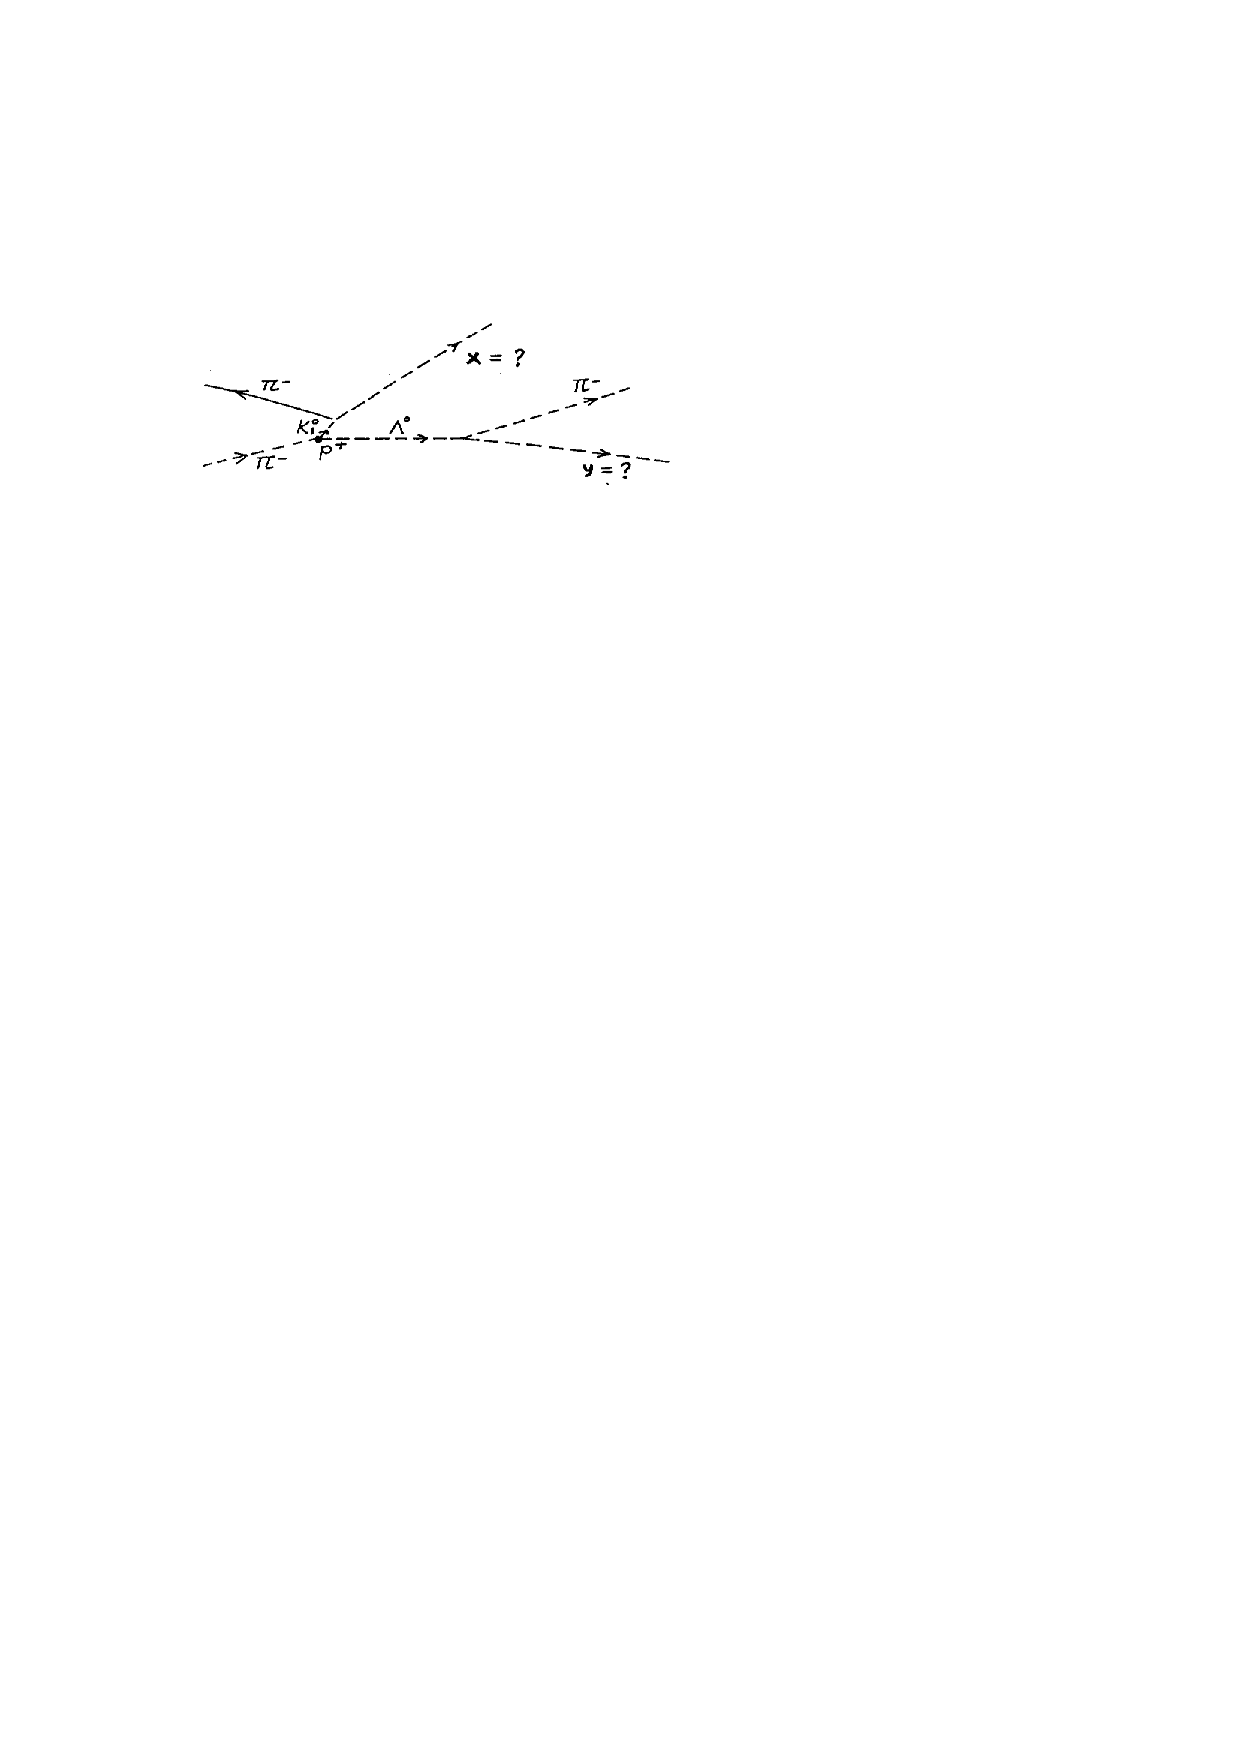
\includegraphics{bellenvat}
    \caption{Bellenvat schets van een foto van de reacties van een pion.}
    \label{fig:bellenvat}
\end{figure}


\question
In BINAS-26 wordt als eenheid van massa vermeld: \si{MeV.c^{-2}}.
\begin{parts}
\part Wat wordt hiermee bedoeld?
\makelines{2}
\part Hoeveel keer zo traag is het muon vergeleken met het electron? Leg uit.
\makelines{2}
\part Hoeveel energie is er minstens nodig om een muon en zijn antideeltje te
creëren? Leg uit.
\makelines{2}
\end{parts}

\question
Het \Ppiplus-meson bestaat uit de quarks \Pup en \APdown.
\begin{parts}
\part Bereken het massadefect bij het combineren van een \Pup met een \APdown quark.
\emph{Binas geeft een indicatie van de quarkmassa! Quarks bestaan niet los!}
\makelines{2}
\part Bereken de bindingsenergie van de quarks in het \Ppiplus-meson.
\makelines{2}
\end{parts}

\question
Gegeven: een reactie waarbij uit één baryon een nieuw baryon én een meson ontstaat:
\ce{\PgD^{++} -> \Pp^+ + \Ppiplus }
\begin{parts}
\part Uit welke quarks bestaan het $\Pp^+$ en \Ppiplus?
\makelines{2}
\part Uit welke quarkcombinatie bestaat het $\PgD^{++}$-deeltje?
\makelines{2}
\uplevel{De massa van het $\PgD^{++}$-deeltje is 1230\si{MeV.c^{-2}}.}
\part Bereken de massa van het $\PgD^{++}$-deeltje, uitgedrukt in kilogram.
\makelines{2}
\part Hoeveel energie komt vrij bij het verval van het $\PgD^{++}$-deeltje?
Geef de berekening.
\makelines{3}
\end{parts}


\uplevel{\section{De zon en neutrino's}}

\question
De energieproductie van een ster is voor een deel afkomstig van kernfusie
(het overige deel is het gevolg van gravitatiecontractie). Voor fusie is in
een ster een overvloed aan waterstofkernen aanwezig. Via een reeks van vier
opeenvolgende stappen wordt waterstof omgezet in helium. Bij de eerste stap
ontstaan onder andere een deuteriumkern en een neutrino:

%\ce{\Pp^+ + \Pp^+ -> ^2_1H + \Pnu + ? } \\
\begin{align}
\cee{ \label{eq:deuterium}
^1_1H+ + ^1_1H+ &-> ^2_1H+ + e^+ + \nu \\
?  + ^2_1H+  &-> ^3_2He^2+ + \gamma \\
^3_2He^2+ + ^3_2He^2+  &-> ^4_2He^2+ + 2\cdot ? \\
e^+ + ? &-> \gamma  \\
}
\end{align}
De laatste stap betreft het ``opruimen'' van de positronen door middel van
annihilatie.
\begin{parts}
\part Wat is in de opeenvolgende stappen de identiteit van de met ``?'' aangegeven deeltjes?
\makelines{3}
\part Hoeveel waterstofkernen zijn (netto) nodig geweest om één heliumkern te vormen?
\makelines{2}
\part Geef de netto-vergelijking voor de productie van één heliumkern.
\makelines{3}
\part Bereken de energie die bij de productie van één heliumatoom vrijkomt.
\makelines{3}
\end{parts}


\question
De energieproductie van onze zon vindt voornamelijk plaats in de kern doordat
waterstofkernen fuseren tot helium.
Bij één fusieproces wordt 26,731 \si{MeV} energie geproduceerd en komen
twee neutrino's vrij.
In \figref{fig:Zonsdoorsnede} zie je een gamma en een neutrino de zon
verlaten. Beide zijn ongeveer geproduceerd op hetzelfde moment.
\begin{figure}[h]
\centering
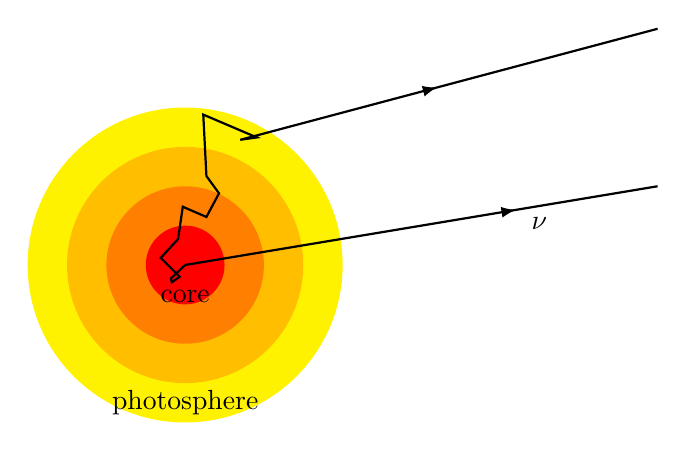
\begin{tikzpicture}[
  particle/.style={thick,decoration={markings, mark=at position .7 with {\arrow[>=latex]{>}}},postaction=decorate}
]
\fill[yellow] (0, 0) circle (2cm);
\fill[orange!50!yellow] (0, 0) circle (1.5cm);
\fill[orange] (0, 0) circle (1cm);
\fill[red] (0, 0) circle (.5cm);

\node at (0, -.4cm) {core};
\node at (0, -1.75cm) {photosphere};

\draw[particle] (0, 0) -- (6cm, 1cm) node[below,near end] {\Pneutrino};
\draw[particle] (0, 0)  -- (-0.18, -0.17)  -- (-0.17, -0.22)  -- (-0.07, -0.15)  -- (-0.31, 0.09)  -- (-0.09, 0.33)  -- (-0.03, 0.74)  -- (0.27, 0.61)  -- (0.43, 0.91)  -- (0.27, 1.13)  -- (0.23, 1.91)  -- (0.91, 1.62)  -- (0.70, 1.59) -- (6cm, 3cm) node[below,near end] {\Pphoton};
\end{tikzpicture}
\caption{Zonsdoorsnede}
\label{fig:Zonsdoorsnede}
\end{figure}
\begin{parts}
\part Leg uit dat het neutrino de zon veel sneller zal verlaten dan het gamma.
\makelines{2}
\part Zoek op in BINAS hoe groot het uitgestraald vermogen van de zon is.
\makelines{2}
\part Bereken het aantal neutrino's dat de zon per seconde uitzendt.
\makelines{5}
\part Bereken de massavermindering van de zon in één jaar.
\makelines{4}
\uplevel{Alle neutrino's verlaten de zon. Ze worden naar alle richtingen uitgezonden.
Op aarde is een neutrinodetector opgesteld met een naar de zon gekeerde
doorsnede van 5,0 m$^{2}$.}
\part Zoek op in BINAS hoe groot de afstand van de detector tot de zon gemiddeld
is.
\makelines{2}
\part Bereken hoeveel neutrino's per seconde de detector bereiken.
\makelines{4}
\end{parts}

\end{questions}
\end{document}
